\documentclass[12pt]{article}

% ── Packages ──────────────────────────────────────────────────────
\usepackage[margin=2.5cm]{geometry}
\usepackage{booktabs}
\usepackage{float}
\usepackage{graphicx}
\usepackage{hyperref}
\usepackage{amsmath}
\usepackage{longtable}
\usepackage{array}
% \usepackage{multirow}
% \usepackage{caption}
% \usepackage{parskip}          % paragraph spacing instead of indent

\floatplacement{figure}{H}

% ── Title ─────────────────────────────────────────────────────────
\title{Are Headtracking Measures an Indicator of Depressive Symptoms? \\[6pt]
       \large Mid-Submission Report — VR 360° Experiment}
\author{}
\date{March 2026}

\begin{document}
\maketitle

% ══════════════════════════════════════════════════════════════════
\section{Introduction}
% ══════════════════════════════════════════════════════════════════

\subsection{Background}

Depression is one of the most prevalent mental health conditions worldwide, affecting approximately 280 million people globally (WHO, 2023). Among its diverse symptomatology, \emph{psychomotor retardation}---a slowing of physical movement and cognitive processing---has long been recognised as a core feature of depressive disorders (American Psychiatric Association, 2013). Behavioural manifestations of psychomotor slowing include reduced exploratory activity, diminished engagement with the environment, and decreased overall movement (Buyukdura et al., 2011).

Virtual Reality (VR) provides an ecologically valid environment for measuring such behaviour because participants interact with immersive environments while their head movements are continuously tracked. Unlike traditional laboratory paradigms that rely on self-report or constrained motor tasks, VR-based headtracking captures naturalistic exploratory behaviour---the degree to which individuals visually scan and orient themselves within an environment (Parsons, 2015).

The present study investigates whether VR headtracking data can reveal behavioural indicators of depressive symptoms. Participants experienced immersive 360° videos while wearing a Meta Quest 3 headset, which recorded head orientation (pitch, yaw, roll) and rotational speed. Alongside the VR experience, participants completed standardised psychological questionnaires measuring depression (PHQ-9), anxiety (GAD-7), trait anxiety (STAI-T), and affect (PANAS).

\subsection{Research Question}

The central research question of this study is:

\begin{quote}
\textbf{Do depressive symptoms influence head-movement behaviour during VR exploration?}
\end{quote}

Understanding this relationship could contribute to the development of digital behavioural markers of mental health that go beyond traditional self-report assessments.

\subsection{Hypotheses}
\begin{itemize}
  \item \textbf{Primary Hypothesis.} Participants with higher PHQ-9 depression scores will exhibit reduced psychomotor activity, reflected in lower mean head rotation speed and reduced variability in head orientation.

  \item \textbf{Secondary Hypothesis.} Higher anxiety scores (GAD-7) may be associated with increased or erratic head scanning behaviour, particularly in emotionally intense environments.

  \item \textbf{Tertiary Hypothesis.} Different VR environments will induce distinct emotional responses (valence and arousal), and these environmental differences may modulate head-movement patterns.


\end{itemize}



% ══════════════════════════════════════════════════════════════════
\section{Methods}
% ══════════════════════════════════════════════════════════════════

\subsection{Participants}

The sample comprised 40 college students (36 male, 4 female; mean age = 22.78 years, \emph{SD} = 1.80, range: 20--28). Participants were recruited through convenience sampling and provided informed consent before taking part in the study. Prior VR experience was recorded using a binary scale (1 = No, 2 = Yes); 24 participants reported prior VR experience, while 16 did not. No participants were excluded from analysis (see Section~3 for exclusion criteria).

\subsection{Experimental Procedure}

Participants viewed five 360° VR videos presented through a Meta Quest 3 headset. Videos were selected to span a range of emotional content:

\begin{table}[H]
\centering
\begin{tabular}{lll}
\toprule
Video & Environment         & Emotional Category \\
\midrule
V1    & Abandoned buildings & Negative           \\
V2    & Evening beach       & Positive           \\
V3    & University campus   & Neutral            \\
V4    & Horror (The Nun)    & High arousal       \\
V5    & Tahiti surf         & Positive           \\
\bottomrule
\end{tabular}
\end{table}

Before the VR experience, participants completed the PHQ-9, GAD-7, STAI-T, and a pre-experiment PANAS. After viewing each video, participants rated the emotional valence (1 = unpleasant, 9 = pleasant) and arousal (1 = calming, 9 = exciting), as well as their sense of immersion/presence. After all videos, participants completed a post-experiment PANAS and the VRISE simulator sickness scale.

During each video, the headset's built-in sensors recorded head orientation and rotational speed at approximately 70\,Hz, yielding time-series data of position changes (X, Y, Z), rotation changes (pitch, yaw, roll), and rotational speed (per axis and total).

\subsection{Psychological Measures}

\begin{itemize}
  \item \textbf{PHQ-9} (Patient Health Questionnaire-9; Kroenke et al., 2001): 9-item depression screening tool. Scores range from 0 to 27; scores $\geq 5$ indicate mild depression, $\geq 10$ moderate depression.
  \item \textbf{GAD-7} (Generalised Anxiety Disorder-7; Spitzer et al., 2006): 7-item anxiety measure. Scores range from 0 to 21.
  \item \textbf{STAI-T} (State-Trait Anxiety Inventory, Trait subscale; Spielberger et al., 1983): 20-item trait anxiety instrument. Scores range from 20 to 80.
  \item \textbf{PANAS} (Positive and Negative Affect Schedule; Watson et al., 1988): measures positive and negative affect pre- and post-VR.
  \item \textbf{VRISE} (Virtual Reality Induced Symptoms and Effects; Sharples et al., 2008): assesses simulator sickness severity.
\end{itemize}

\subsection{Head-Tracking Metrics}

From the raw headtracking time-series, the following movement features were computed for each participant--video combination:

\textbf{Primary metrics:}

\begin{itemize}
  \item \emph{Mean rotation speed} (°/s): the average total rotational speed across the recording, reflecting the overall level of exploratory head movement.
  \item \emph{SD of yaw} (°): the standard deviation of horizontal head rotation, capturing left--right scanning variability.
  \item \emph{SD of pitch} (°): the standard deviation of vertical head rotation, capturing up--down scanning variability.
\end{itemize}

\textbf{Secondary metrics:}

\begin{itemize}
  \item \emph{SD of roll} (°): the standard deviation of head tilt.
  \item \emph{Total movement magnitude}: the cumulative sum of absolute rotation changes across all axes ($\sum |\Delta X| + |\Delta Y| + |\Delta Z|$), quantifying total displacement.
\end{itemize}

Data pre-processing involved filtering malformed CSV records, converting columns to numeric, and removing incomplete samples. Files with fewer than 10 valid samples were excluded.

\subsection{Participant Grouping}

Participants were categorised into two groups based on their PHQ-9 depression scores, using the clinically validated cutoff of $\geq 5$ (Kroenke et al., 2001):

\begin{table}[H]
\centering
\begin{tabular}{lcc}
\toprule
Group           & PHQ-9 Range & \emph{n} \\
\midrule
Non-Depressed   & 0--4        & 20       \\
Depressed       & $\geq 5$    & 20       \\
\bottomrule
\end{tabular}
\end{table}

This threshold identifies participants with at least \emph{mild} depressive symptomatology. A secondary cutoff of $\geq 10$ (moderate depression; \emph{n} = 8 vs.\ 32) was used for sensitivity analysis.

\subsection{Statistical Analysis}

All analyses were conducted in R (version 4.5.2; R Core Team, 2025). The analysis pipeline proceeded as follows:

\begin{itemize}
  \item \textbf{Descriptive statistics and distributional checks.} For each psychological scale and headtracking metric, means, standard deviations, medians, and interquartile ranges were computed. Shapiro-Wilk tests assessed normality of the headtracking variables. Distribution shapes were inspected via density plots and Q-Q plots.
  
  \item \textbf{Outlier detection.} Potential outliers on headtracking variables were identified using two criteria: (a) values exceeding $1.5 \times \text{IQR}$ beyond the 25th or 75th percentile, and (b) standardised \emph{z}-scores exceeding $\pm 2.5$. Outliers based on VRISE scores were examined, but no participants were excluded from the final analysis.
  
  \item \textbf{Group comparison (primary hypothesis test).} For each metric $\times$ video combination (25 comparisons total), the non-depressed and depressed groups were compared. When both groups passed the Shapiro-Wilk normality test ($p > .05$), Welch's \emph{t}-test was employed; otherwise, the Mann-Whitney \emph{U} test was used. Cohen's \emph{d} was computed as the effect size. To correct for multiple comparisons, Benjamini-Hochberg false discovery rate (FDR) adjustment was applied.
  
  \item \textbf{Correlation analysis.} Pearson correlations assessed the bivariate relationship between PHQ-9 scores and averaged headtracking metrics. The comorbidity between depression and anxiety was examined via the PHQ-9--GAD-7 correlation.
  
  \item \textbf{Within-subjects video effects.} Friedman tests assessed whether headtracking metrics differed significantly across the five videos. Post-hoc pairwise Wilcoxon signed-rank tests with Bonferroni correction were conducted for significant omnibus results. A Kruskal-Wallis test further compared headtracking metrics across emotional video categories (positive, neutral, negative).
  
\end{itemize}


% % ══════════════════════════════════════════════════════════════════
% \section{Data Preparation and Preliminary Checks}
% % ══════════════════════════════════════════════════════════════════

\subsection{Missing Data and Exclusions}

All 40 participants had complete survey data and headtracking recordings for videos V1--V4. Two participants had missing headtracking data for V5 (filenames did not match). Missing data on text-response fields (emotional descriptions, feedback) did not affect quantitative analyses. Three participants (IDs 21, 25, 35) had relatively low VRISE scores (17, 20, and 24, respectively), indicating minimal simulator sickness; their headtracking recordings appeared valid and no sensor artifacts were observed. With only $N = 40$, excluding participants would substantially reduce statistical power. Therefore, all 40 participants were retained for analysis.

\subsection{Outlier Inspection}

Headtracking variables were screened using standard IQR-based criteria, and the few observations that fell outside the expected range were reviewed. No data were excluded due to recording artefacts.

% ══════════════════════════════════════════════════════════════════
\section{Results}
% ══════════════════════════════════════════════════════════════════

\subsection{Descriptive Statistics}

\subsubsection{Psychological Measures}

The sample exhibited a range of depressive symptomatology: mean PHQ-9 = 6.03 (\emph{SD} = 4.63, median = 4.50, range: 0--18). The distribution was positively skewed, with the majority of participants in the minimal-to-mild range. Mean GAD-7 was 5.00 (\emph{SD} = 4.31), and mean STAI-T was 45.00 (\emph{SD} = 14.63), reflecting generally low-to-moderate anxiety. Mean VRISE was 31.88 (\emph{SD} = 3.98); higher VRISE scores correspond to more severe simulator sickness symptoms, so this indicates that most participants reported low-to-moderate discomfort.

\begin{figure}[H]
\centering
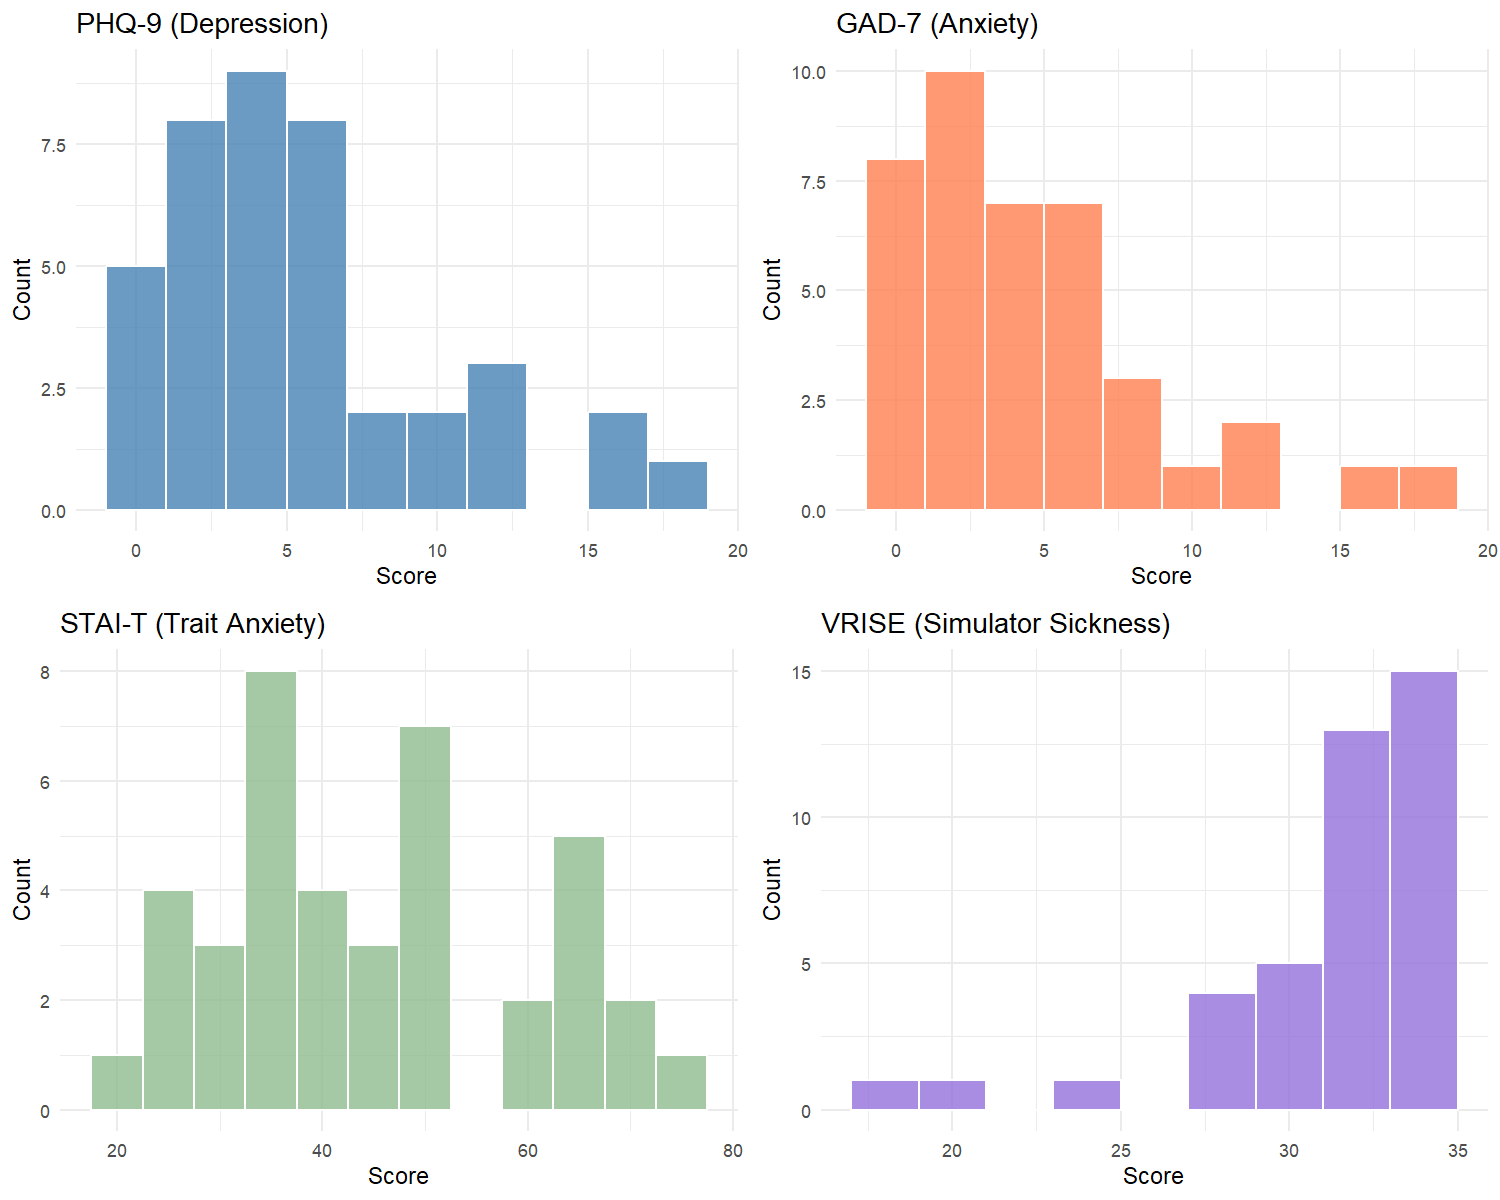
\includegraphics[width=0.5\textwidth]{analysis/output/figures/fig1_psych_scales_histograms.png}
\caption{Distributions of psychological scales across 40 participants. PHQ-9 shows a positive skew; most participants fall in the minimal-to-mild depression range.}
\label{fig:psych}
\end{figure}

\begin{figure}[H]
\centering
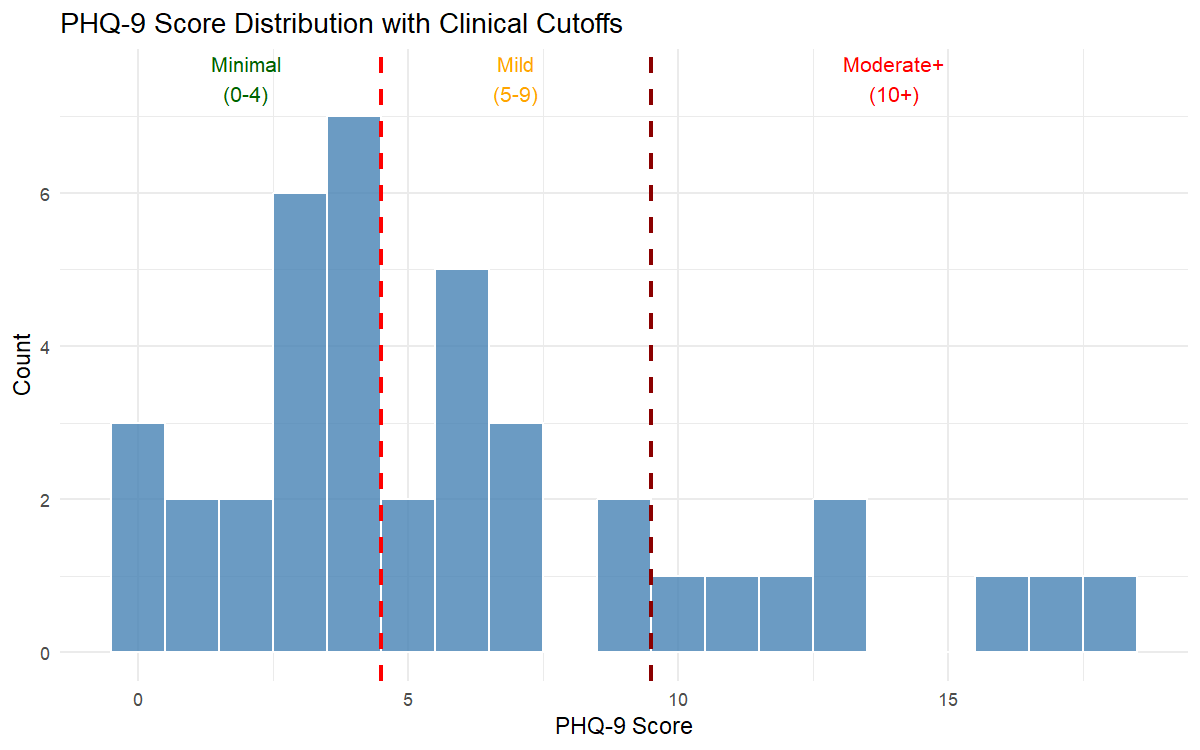
\includegraphics[width=0.5\textwidth]{analysis/output/figures/fig9_phq9_distribution.png}
\caption{PHQ-9 score distribution with clinical cutoff thresholds. Dashed lines indicate the boundaries for Minimal (0--4), Mild (5--9), and Moderate+ ($\geq$10) categories.}
\label{fig:phq9}
\end{figure}

Using the PHQ-9 $\geq 5$ cutoff produced two balanced groups (Non-Depressed: \emph{n} = 20, \emph{M} = 2.60; Depressed: \emph{n} = 20, \emph{M} = 9.45). As expected, the depressed group also scored higher on GAD-7 (\emph{M} = 7.05 vs.\ 2.95) and STAI-T (\emph{M} = 52.25 vs.\ 37.75), consistent with well-documented comorbidity between depression and anxiety.

\subsubsection{Headtracking Measures}

Mean rotation speed varied across videos, with V1 (Abandoned) eliciting the highest overall speed (\emph{M} = 39.09°/s, \emph{SD} = 10.84) and V4 (Horror) the lowest (\emph{M} = 24.17°/s, \emph{SD} = 11.08). Table~\ref{tab:ht} summarises headtracking metrics by video.

\begin{table}[H]
\centering
\caption{Headtracking summary statistics by video.}
\label{tab:ht}
\begin{tabular}{lcccc}
\toprule
Video          & Mean Speed (°/s) & \emph{SD} & SD Yaw (°) & SD Pitch (°) \\
\midrule
V1: Abandoned  & 39.09 & 10.84 & 90.0 & 17.0 \\
V2: Beach      & 32.76 & 9.09  & 88.0 & 11.5 \\
V3: Campus     & 34.88 & 10.48 & 90.0 & 13.0 \\
V4: Horror     & 24.17 & 11.08 & 33.0 & 13.5 \\
V5: Surf       & 31.16 & 11.57 & 85.0 & 13.5 \\
\bottomrule
\end{tabular}
\end{table}

Shapiro-Wilk tests on the participant-level averages (across videos) indicated that mean speed ($W = 0.977$, $p = .584$) and SD of pitch ($W = 0.973$, $p = .438$) were normally distributed, while SD of yaw was significantly non-normal ($W = 0.914$, $p = .005$). SD of roll was marginally normal ($W = 0.948$, $p = .064$).


\subsection{Correlation Analysis}

\subsubsection{PHQ-9 and Headtracking}

A Pearson correlation between PHQ-9 scores and the average mean rotation speed (across all videos) yielded a non-significant result: $r = -.063$, $p = .697$. This indicates that at the aggregate level, there is no meaningful linear relationship between depression severity and overall head-movement speed.

The full correlation matrix (Figure~\ref{fig:corr}) reveals the internal associations among psychological and headtracking variables. PHQ-9 correlated strongly with GAD-7 ($r = .58$, $p < .001$) and STAI-T ($r = .64$, $p < .001$), reflecting the known comorbidity. Pre-experiment negative affect (PANAS-) showed a moderate negative correlation with average speed ($r = -.32$, $p = .042$), suggesting that participants reporting higher negative mood exhibited slightly less head movement.

\begin{figure}[H]
\centering
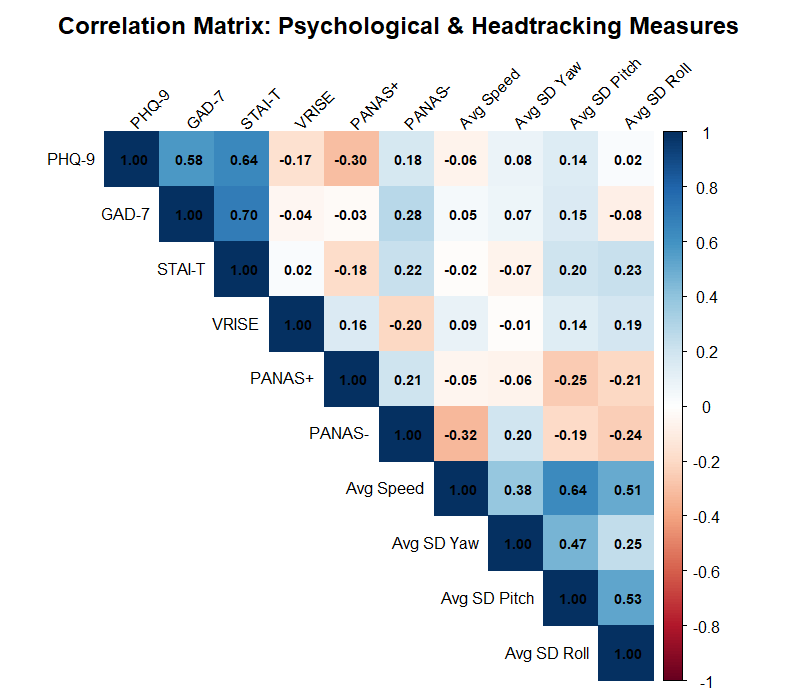
\includegraphics[width=0.5\textwidth]{analysis/output/figures/fig5_correlation_matrix.png}
\caption{Correlation matrix showing relationships among psychological measures and averaged headtracking metrics. PHQ-9 is strongly associated with GAD-7 and STAI-T, but only weakly related to headtracking measures.}
\label{fig:corr}
\end{figure}


\subsection{Group Comparison: Depression and Head Movement}

The core hypothesis was tested by comparing the Non-Depressed (\emph{n} = 20) and Depressed (\emph{n} = 20) groups on each headtracking metric for each video (25 tests total). None of the comparisons reached statistical significance at $p < .05$ (uncorrected), and all Benjamini-Hochberg adjusted \emph{p}-values exceeded .88.

Several medium-sized effects were observed despite the lack of significance:

\begin{itemize}
  \item \textbf{V5 (Surf), Mean Speed:} Non-Depressed \emph{M} = 34.35°/s vs.\ Depressed \emph{M} = 28.12°/s, Welch's \emph{t}-test $p = .105$, $d = 0.54$ (medium).
  \item \textbf{V4 (Horror), SD Yaw:} Non-Depressed \emph{M} = 37.12° vs.\ Depressed \emph{M} = 29.01°, Mann-Whitney $p = .239$, $d = -0.55$ (medium).
  \item \textbf{V4 (Horror), Total Movement:} Mann-Whitney $p = .120$, $d = -0.54$ (medium).
\end{itemize}

\begin{figure}[H]
\centering
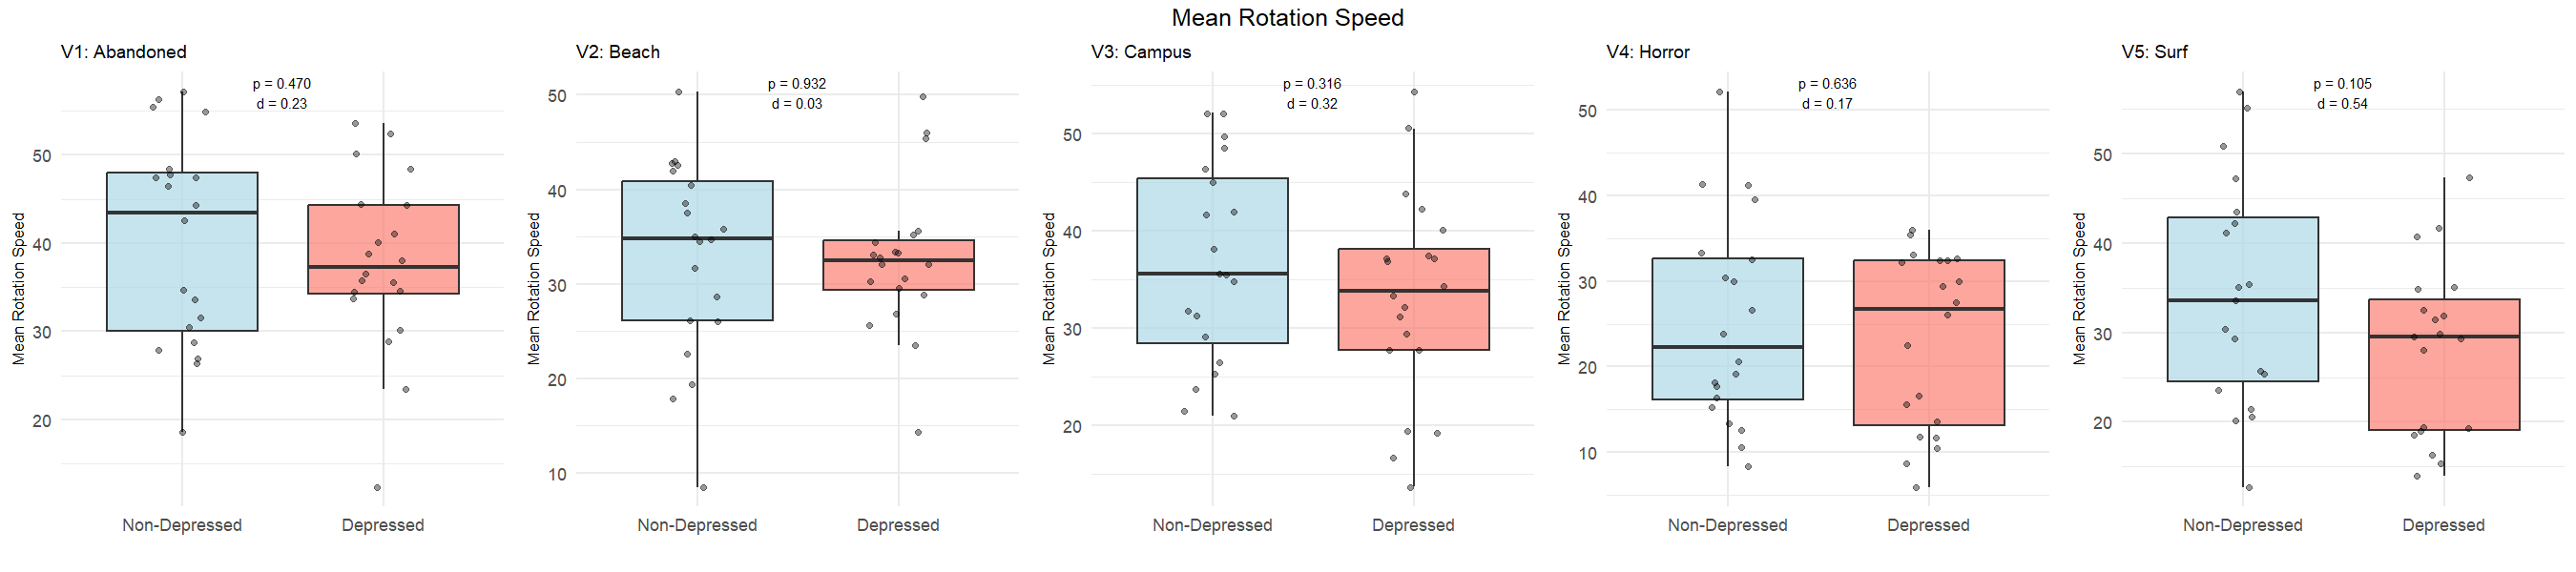
\includegraphics[width=0.7\textwidth]{analysis/output/figures/fig10_group_comparison_mean_speed.png}
\caption{Group comparison for mean rotation speed across five videos. Non-Depressed (blue) vs.\ Depressed (red) groups. No comparison reached statistical significance.}
\label{fig:groupspeed}
\end{figure}

\begin{figure}[H]
\centering
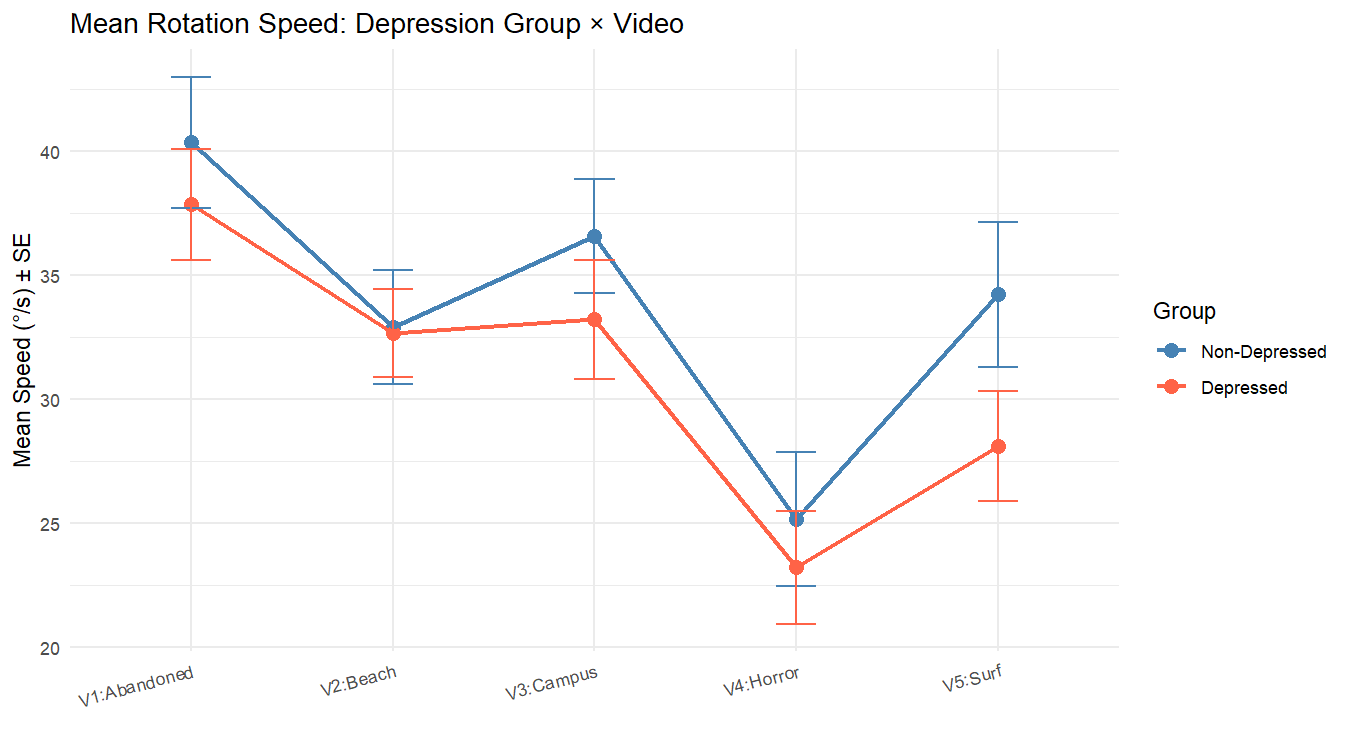
\includegraphics[width=0.5\textwidth]{analysis/output/figures/fig13_interaction_plot.png}
\caption{Interaction plot showing mean rotation speed ($\pm$ SE) for each depression group across the five videos. Both groups show the same pattern of lowest speed during V4 (Horror). The depressed group tends to show lower speed, particularly for V5 (Surf).}
\label{fig:interact}
\end{figure}


\subsection{Emotional Response Across Videos}

\subsubsection{Valence and Arousal Ratings}

The five videos elicited clearly differentiated emotional responses (Figure~\ref{fig:valaro}). V5 (Surf) received the highest valence rating (\emph{M} = 7.12) and arousal (\emph{M} = 6.50), placing it in the ``Excited/Happy'' quadrant of the circumplex model. V4 (Horror) had the lowest valence (\emph{M} = 3.67) but high arousal (\emph{M} = 5.95), corresponding to the ``Tense/Stressed'' quadrant. V2 (Beach) and V3 (Campus) fell in the moderately positive range.

\begin{figure}[H]
\centering
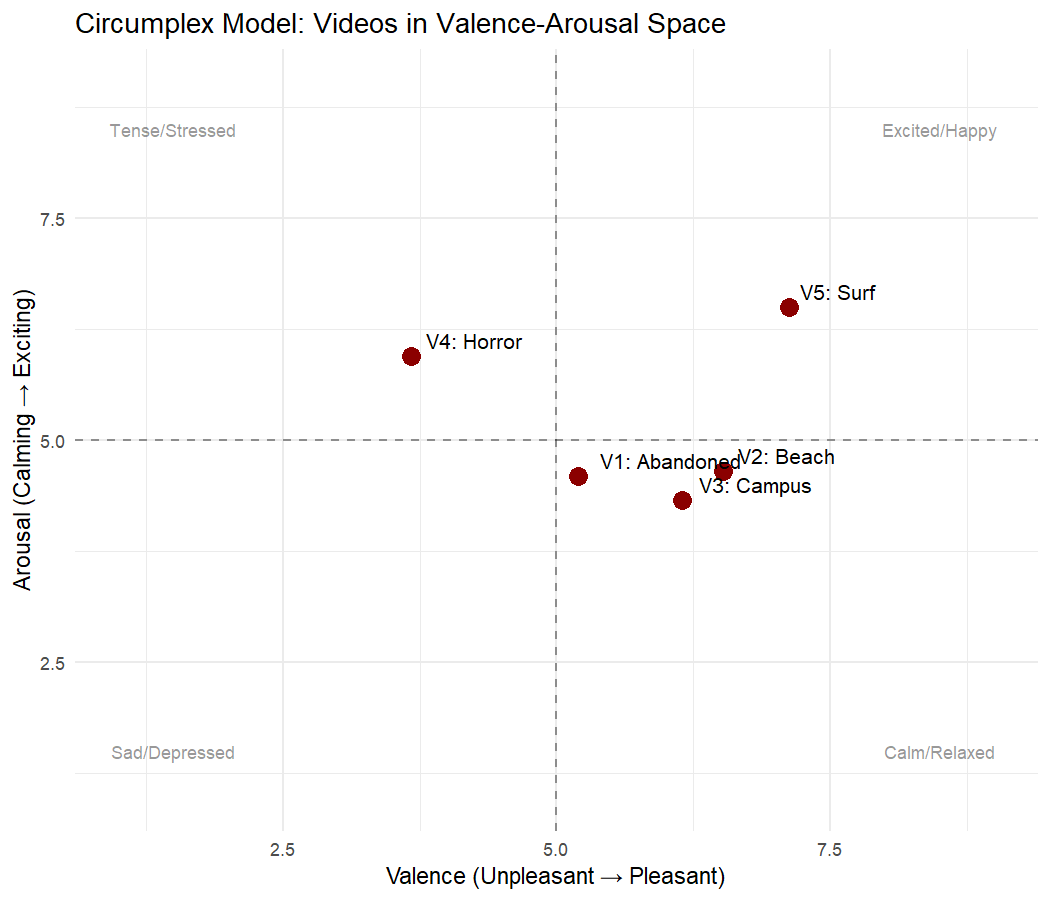
\includegraphics[width=0.5\textwidth]{analysis/output/figures/fig3_circumplex_model.png}
\caption{Circumplex model placing each video's mean valence and arousal ratings. V4 (Horror) and V5 (Surf) occupy high-arousal quadrants; V1, V2, and V3 cluster near the neutral midpoint.}
\label{fig:circ}
\end{figure}


\subsubsection{Video Effects on Head Movement (Friedman Tests)}

Friedman tests revealed highly significant differences in headtracking metrics across the five videos:

\begin{itemize}
  \item \textbf{Mean rotation speed:} $\chi^2(4) = 66.76$, $p < .001$
  \item \textbf{SD of yaw:} $\chi^2(4) = 91.75$, $p < .001$
  \item \textbf{SD of pitch:} $\chi^2(4) = 54.48$, $p < .001$
\end{itemize}

Post-hoc Wilcoxon signed-rank tests (Bonferroni-corrected) showed that V4 (Horror) differed significantly from all other videos on both mean speed and SD of yaw. This is consistent with the constrained visual focus elicited by the horror content (narrow field of interest, freezing behaviour).

\begin{figure}[H]
\centering
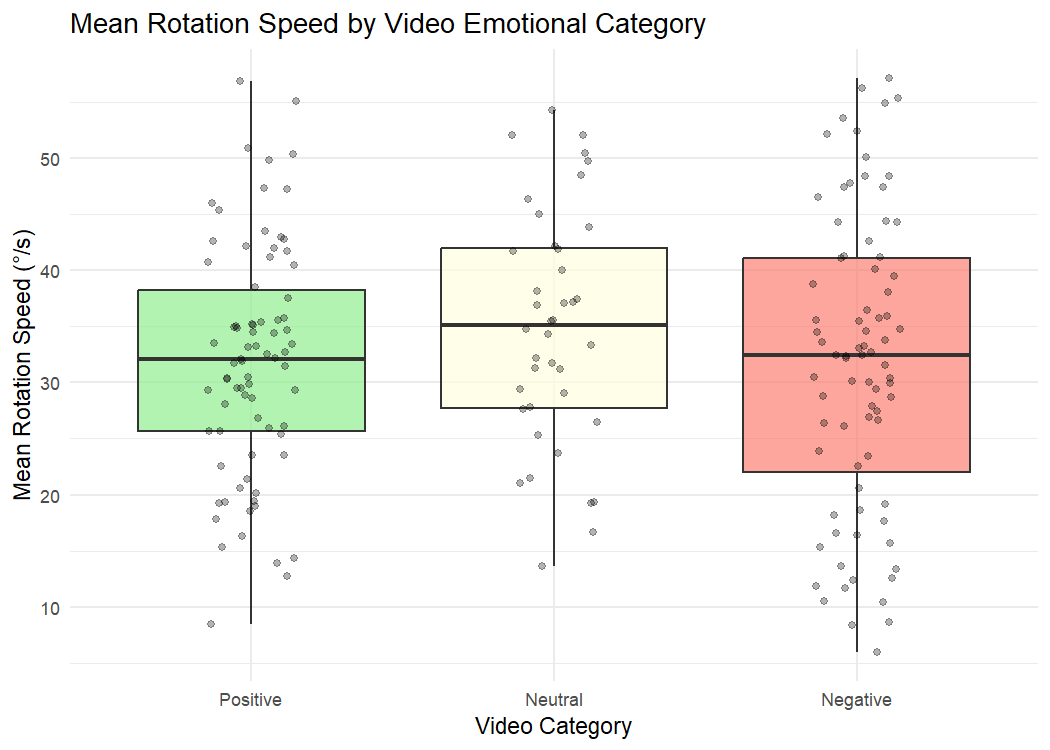
\includegraphics[width=0.5\textwidth]{analysis/output/figures/fig12_speed_by_category.png}
\caption{Mean rotation speed by emotional video category. Horror-related videos (Negative) show reduced movement compared to Positive and Neutral content.}
\label{fig:category}
\end{figure}


% ══════════════════════════════════════════════════════════════════
\section{Discussion}
% ══════════════════════════════════════════════════════════════════

\subsection{Summary of Findings}

This mid-submission report presents the initial statistical analyses for a study investigating whether VR headtracking measures are associated with depressive symptoms. The key findings are:

\begin{enumerate}
  \item \textbf{No statistically significant group differences} were found between participants with low (PHQ-9 $< 5$) and elevated (PHQ-9 $\geq 5$) depressive symptoms on any headtracking metric, across any video. However, several comparisons yielded medium effect sizes ($d \approx 0.5$), particularly for V5 (Surf) mean speed and V4 (Horror) yaw variability and total movement.

  \item The \textbf{zero-order correlation} between PHQ-9 scores and average mean rotation speed was negligible ($r = -.063$, $p = .697$), providing no evidence for a linear relationship at the aggregate level.

  \item \textbf{Video type had a strong effect} on head-movement patterns. Friedman tests were highly significant ($p < .001$) for all three primary metrics. V4 (Horror) consistently produced the lowest movement speed and reduced yaw variability, likely reflecting a constrained scanning pattern during threatening content.

  \item The five videos \textbf{successfully induced differentiated emotional states}, as confirmed by valence and arousal ratings spanning the circumplex model.
\end{enumerate}

\subsection{Interpretation}

The absence of significant group differences may be attributable to several factors. First, the sample size ($N = 40$) provides limited statistical power. A post-hoc power analysis for the observed effect of $d = 0.54$ with two groups of 20 yields a power of approximately .37 ($\alpha = .05$, two-tailed), well below the conventional .80 threshold. Second, the PHQ-9 distribution was skewed toward lower scores (median = 4.5), meaning that even the ``depressed'' group largely comprised participants with mild symptomatology rather than clinical depression.

The medium effect sizes observed---particularly during high-arousal (V5: Surf) and high-threat (V4: Horror) videos---suggest that emotionally salient contexts may amplify behavioural differences between depression groups. This aligns with theories of emotional context insensitivity in depression (Rottenberg, 2005), where individuals with depressive symptoms show blunted responses to both positive and negative stimuli.

\subsection{Limitations}

The main limitations of the current analysis include (a) the small sample size reducing power to detect small-to-medium effects, (b) a predominantly male sample (90\% male) limiting generalisability, (c) reliance on self-report depression screening rather than clinical diagnosis, and (d) the lack of counterbalanced video presentation order.


% ══════════════════════════════════════════════════════════════════
\section{Future Work (Final Report)}
% ══════════════════════════════════════════════════════════════════

The final report will extend the present analysis with the following:

\begin{itemize}
  \item \textbf{Partial correlations} controlling for anxiety (GAD-7, STAI-T) to isolate the unique contribution of depression.
  \item \textbf{Stratified analysis} examining depression effects within low- and high-anxiety subgroups.
  \item \textbf{PANAS pre/post comparisons} to assess affective change during the VR experience.
  \item \textbf{Immersion and presence} correlations with headtracking, to determine whether engagement moderates movement.
  \item \textbf{Sensitivity analysis} using the stricter PHQ-9 $\geq 10$ cutoff.
  \item \textbf{Multiple comparison correction} with more thorough exploration of interaction effects.
\end{itemize}

% ══════════════════════════════════════════════════════════════════
\section{Author Contributions}
% ══════════════════════════════════════════════════════════════════

All team members contributed equally to the design of the experiment, preprocessing of the data, statistical analysis, generation of figures, and writing of this report.


\begin{thebibliography}{99}

\bibitem{apa2013}
American Psychiatric Association. (2013). \emph{Diagnostic and statistical manual of mental disorders} (5th ed.). American Psychiatric Publishing.

\bibitem{buyukdura2011}
Buyukdura, J. S., McClintock, S. M., \& Croarkin, P. E. (2011). Psychomotor retardation in depression: Biological underpinnings, measurement, and treatment. \emph{Progress in Neuro-Psychopharmacology and Biological Psychiatry, 35}(2), 395--409.

\bibitem{kroenke2001}
Kroenke, K., Spitzer, R. L., \& Williams, J. B. (2001). The PHQ-9: Validity of a brief depression severity measure. \emph{Journal of General Internal Medicine, 16}(9), 606--613.

\bibitem{parsons2015}
Parsons, T. D. (2015). Virtual reality for enhanced ecological validity and experimental control in the clinical, affective and social neurosciences. \emph{Frontiers in Human Neuroscience, 9}, 660.

\bibitem{rcore2025}
R Core Team. (2025). \emph{R: A language and environment for statistical computing}. R Foundation for Statistical Computing.

\bibitem{rottenberg2005}
Rottenberg, J. (2005). Mood and emotion in major depression. \emph{Current Directions in Psychological Science, 14}(3), 167--170.

\bibitem{sharples2008}
Sharples, S., Cobb, S., Moody, A., \& Wilson, J. R. (2008). Virtual reality induced symptoms and effects (VRISE): Comparison of head mounted display (HMD), desktop and projection display systems. \emph{Displays, 29}(2), 58--69.

\bibitem{spielberger1983}
Spielberger, C. D., Gorsuch, R. L., Lushene, R., Vagg, P. R., \& Jacobs, G. A. (1983). \emph{Manual for the State-Trait Anxiety Inventory}. Consulting Psychologists Press.

\bibitem{spitzer2006}
Spitzer, R. L., Kroenke, K., Williams, J. B. W., \& L\"{o}we, B. (2006). A brief measure for assessing generalized anxiety disorder: The GAD-7. \emph{Archives of Internal Medicine, 166}(10), 1092--1097.

\bibitem{watson1988}
Watson, D., Clark, L. A., \& Tellegen, A. (1988). Development and validation of brief measures of positive and negative affect: The PANAS scales. \emph{Journal of Personality and Social Psychology, 54}(6), 1063--1070.

\bibitem{who2023}
World Health Organization. (2023). \emph{Depressive disorder (depression): Fact sheet}. Retrieved from \url{https://www.who.int/news-room/fact-sheets/detail/depression}

\end{thebibliography}
\end{document}
